\documentclass[11pt,
			   %10pt, 
               %hyperref={colorlinks},
               aspectratio=169,
               hyperref={colorlinks}
               ]{beamer}
\usetheme{Singapore}
\usecolortheme[snowy, cautious]{owl}

\usepackage[utf8]{inputenc}
\usepackage[T1]{fontenc}
\usepackage[american]{babel}
\usepackage{graphicx}
\usepackage{hyperref}
\hypersetup{
    colorlinks=true,
    urlcolor=[rgb]{1,0,1},
    linkcolor=[rgb]{1,0,1}}

\usepackage[natbib=true,style=authoryear,backend=bibtex,useprefix=true]{biblatex}

%\setbeamercolor*{bibliography entry title}{fg=black}
%\setbeamercolor*{bibliography entry location}{fg=black}
%\setbeamercolor*{bibliography entry note}{fg=black}
\definecolor{OwlGreen}{RGB}{75,0,130} % easier to see
\setbeamertemplate{bibliography item}{}
\setbeamerfont{caption}{size=\footnotesize}
\setbeamertemplate{frametitle continuation}{}
\setcounter{tocdepth}{1}
\renewcommand*{\bibfont}{\scriptsize}
\addbibresource{lecture_6.bib}

\renewcommand*{\thefootnote}{\fnsymbol{footnote}}

\usenavigationsymbolstemplate{}
\setbeamertemplate{footline}{%
    \raisebox{5pt}{\makebox{\hfill\makebox[20pt]{\color{gray}
          \scriptsize\insertframenumber}}}\hspace*{5pt}}

\author{Patrick Hall}
\title{Lecture 6: Responsible Machine Learning Best Practices\footnote{\tiny{This material is shared under a \href{https://creativecommons.org/licenses/by/4.0/deed.ast}{CC By 4.0 license} which allows for editing and redistribution, even for commercial purposes. However, any derivative work should attribute the author.}}}
\institute{The George Washington University}
\date{\today}

\begin{document}
	
	\maketitle
	
	\begin{frame}
	
		\frametitle{Contents}
		
		\tableofcontents{}
		
	\end{frame}

%-------------------------------------------------------------------------------
	\section{Blueprint}
%-------------------------------------------------------------------------------
	
		\begin{frame}
		
			\frametitle{Preface}			
			
			This mid-level technical document provides a basic blueprint for combining innovations in AutoML, regulation-compliant predictive modeling, and machine learning research in the sub-disciplines of fairness, interpretable models, post-hoc explanations, privacy and security to create a low-risk machine learning framework.\\
			
			\vspace{10pt}			
			
			This document presents potential technical solutions to the \textbf{intersectional} harms posed by opaqueness, inaccuracy, social bias, or security vulnerabilities in machine learning.
			
			\vspace{10pt}
			
			Racism, sexism, cyber-crime and other issues discussed in this document have not been solved, and likely cannot be solved, by technology alone.  
			
		\end{frame}					
		
		\begin{frame}				
		
			\frametitle{Blueprint\footnote{\tiny{This blueprint does not address ETL workflows.}}}
							
			\begin{figure}[htb]
				\begin{center}
					\includegraphics[height=150pt]{../img/blueprint.png}
					\label{fig:blueprint}
				\end{center}
			\end{figure}		
		
		\end{frame}

%-------------------------------------------------------------------------------
	\section{EDA}
%-------------------------------------------------------------------------------
	
		\begin{frame}
		
			\frametitle{EDA and Data Visualization}		
			
			\begin{columns}
	
				\column{0.5\linewidth}
				\centering
				\includegraphics[height=120pt]{../img/eda.png}
				
				\column{0.5\linewidth}
				\vspace{-5pt}
				\begin{itemize}
					\item Know thy data.
					%\item \textbf{Automation} implemented in Driverless AI as AutoViz.
					\item OSS: \href{http://docs.h2o.ai/h2o/latest-stable/h2o-docs/data-science/aggregator.html}{H2O-3 Aggregator}
					\item References: \citefield{wilkinson2018visualizing}{title}; \citefield{wilkinson2006grammar}{title}
				\end{itemize}
				
			\end{columns}
		
		\end{frame}
		
%-------------------------------------------------------------------------------
		\subsection{My Favorites}
%-------------------------------------------------------------------------------		
		
			\begin{frame}

				\frametitle{Interlude: My Favorite Visualizations}		
			
				\vspace{-15pt}
			
				\begin{columns}
	
					\column{0.5\linewidth}
					\centering
					\includegraphics[height=160pt]{../img/net_graph.png}
					
					\tiny{A network graph capturing the Pearson correlation relationships between many \textit{columns} in a lending dataset.}
				
					\column{0.5\linewidth}
					
					\vspace{19pt}
					\centering
					\includegraphics[height=120pt]{../img/ae.png}
					
					\vspace{19pt}
					
					\tiny{An autoencoder projection of the MNIST data. Projections capture sparsity, clusters, hierarchy, and outliers in \textit{rows} of a dataset.}
				
				\end{columns}
			
				\vspace{10pt}
			
				\centering
				\footnotesize{Both of these images capture high-dimensional datasets in just two dimensions.}
		
			\end{frame}

%-------------------------------------------------------------------------------
	\section{Benchmark}
%-------------------------------------------------------------------------------
	
		\begin{frame}
		
			\frametitle{Establish Benchmarks}		

			\begin{figure}[htb]
				\begin{center}
					\includegraphics[height=135pt]{../img/bench.png}
				\end{center}
			\end{figure}	

			\vspace{-10pt}
			\scriptsize{Establishing reproducible benchmarks from which to gauge improvements in accuracy, fairness, interpretability or privacy is crucial for good (``data'') science and for compliance. }
		
		\end{frame}


%-------------------------------------------------------------------------------
	\section{Training}
%-------------------------------------------------------------------------------

%-------------------------------------------------------------------------------
		\subsection{Feature Engineering}
%-------------------------------------------------------------------------------

			\begin{frame}
		
				\frametitle{Manual, Private, Sparse or Straightforward Feature Engineering }		
		
				\begin{columns}
	
					\column{0.5\linewidth}
					\centering
					\includegraphics[height=120pt]{../img/fe.png}
				
					\column{0.5\linewidth}
					\vspace{-5pt}
					\begin{itemize}
						\item OSS: \href{https://cran.r-project.org/web/packages/elasticnet/index.html}{elasticnet}, \href{https://index.pocketcluster.io/featuretools-featuretools.html}{Feature Tools}
						\item References: \citefield{zou2006sparse}{title}; \citefield{kanter2016label}{title}; \citefield{t_closeness}{title}
					\end{itemize}
				
				\end{columns}		
		
			\end{frame}
	
%-------------------------------------------------------------------------------
		\subsection{Preprocessing}
%-------------------------------------------------------------------------------	
	
			\begin{frame}
		
				\frametitle{Preprocessing for Fairness, Privacy or Security}		
			
				\begin{columns}
	
					\column{0.5\linewidth}
					\centering
					\includegraphics[height=120pt]{../img/pre.png}
				
					\column{0.5\linewidth}
					\vspace{-5pt}
					\begin{itemize}
						\item OSS: IBM \href{https://github.com/IBM/AIF360}{AIF360}
						\item References: \citefield{kamiran2012data}{title}; \citefield{feldman2015certifying}{title}; \citefield{calmon2017optimized}{title}; \citefield{agrawal2000privacy}{title}; \citefield{ji2014differential}{title}
					\end{itemize}
				
				\end{columns}			
			
			\end{frame}
			
%-------------------------------------------------------------------------------
		\subsection{Interpretable Models}
%-------------------------------------------------------------------------------			
			
			\begin{frame}
		
				\frametitle{Constrained, Fair, Interpretable, Private or Simple Models}		
			
				\begin{columns}
	
					\column{0.5\linewidth}
					\centering
					\includegraphics[height=120pt]{../img/im.png}
				
					\column{0.5\linewidth}
					\vspace{-5pt}
					\small
					\begin{itemize}
						\item OSS: \href{https://github.com/interpretml/interpret}{\citefield{ga2m}{title} (GA2M/EBM)}; \href{https://users.cs.duke.edu/~cynthia/code.html}{Rudin Group models} e.g. \citefield{sbrl}{title} (SBRL); Monotonic gradient boosting machines in \href{https://github.com/h2oai/h2o-3/blob/master/h2o-py/demos/H2O_tutorial_gbm_monotonicity.ipynb}{H2O-3} or \href{https://xiaoxiaowang87.github.io/monotonicity_constraint/}{XGBoost}; \href{https://docs.pymc.io/}{pymc3}
						\item References: \citefield{pate}{title}; \citefield{zhang2018mitigating}{title}; \citefield{pearl2011bayesian}{title}; \citefield{wf_xnn}{title} (XNN)
					\end{itemize}
					\normalsize
				
				\end{columns}			
			
			\end{frame}

%-------------------------------------------------------------------------------
	\section{Post-Hoc Analysis}
%-------------------------------------------------------------------------------

%-------------------------------------------------------------------------------
		\subsection{Calibration}
%-------------------------------------------------------------------------------			

			\begin{frame}
		
				\frametitle{Prediction Calibration}		
			
				\begin{columns}
	
					\column{0.5\linewidth}
					\centering
					\includegraphics[height=120pt]{../img/calibrate.png}
				
					\column{0.5\linewidth}
					\begin{itemize}
						\item Just because a number is in $[0,1]$ does not make it a probability. 
						\item OSS: \href{https://scikit-learn.org/stable/modules/calibration.html}{scikit-learn} 
						\item References: \citefield{niculescu2005predicting}{title}
					\end{itemize}
				
				\end{columns}			

			\end{frame}

%-------------------------------------------------------------------------------
		\subsection{Model Assessment}
%-------------------------------------------------------------------------------			

			\begin{frame}
		
				\frametitle{Traditional Model Assessment and Diagnostics}		
			
				\begin{figure}[htb]
					\begin{center}
						\includegraphics[height=135pt]{../img/ma.png}
					\end{center}
				\end{figure}	

			\vspace{-10pt}
			\scriptsize{Residual analysis, Q-Q plots, AUC and lift curves etc. confirm model is accurate and meets assumption criteria.}
		
			\end{frame}

%-------------------------------------------------------------------------------
		\subsection{Post-hoc Explanations}
%-------------------------------------------------------------------------------			
			
			\begin{frame}
		
				\frametitle{Post-hoc Explanations}		
			
				\begin{columns}
	
					\column{0.5\linewidth}
					\centering
					\includegraphics[height=120pt]{../img/exp.png}
				
					\column{0.5\linewidth}
					\vspace{-5pt}
					
					\small{
					\begin{itemize}
						\item Explanations enable \textit{understanding} and \textit{appeal} ... \textit{not trust}.
						\item OSS: \href{https://github.com/SeldonIO/alibi}{alibi}, \href{https://github.com/slundberg/shap}{shap} 
						\item References: \citefield{wachter2017counterfactual}{title}; \citefield{shapley}{title}; \citefield{dt_surrogate2}{title}; \citefield{please_stop}{title} (criticism)
					\end{itemize}}
				
				\end{columns}
		
			\end{frame}

			\begin{frame}
		
				\frametitle{Interlude: The Time--Tested Shapley Value}		
			
				\begin{enumerate}
				
					\item \textbf{In the beginning}: \citefield{shapley1953value}{title}, \citefield{shapley1953value}{year}
					\item \textbf{Nobel-worthy contributions}: \citefield{shapley1988shapley}{title}, \citefield{shapley1988shapley}{year}
					\item \textbf{Shapley regression}: \citefield{lipovetsky2001analysis}{title}, \citefield{lipovetsky2001analysis}{year}
					\item \textbf{First reference in ML?} \citefield{keinan2004fair}{title}, \citefield{keinan2004fair}{year} 	
					\item \textbf{Into the ML research mainstream, i.e. JMLR}: \citefield{kononenko2010efficient}{title}, \citefield{kononenko2010efficient}{year}
					\item \textbf{Into the real-world data mining workflow ... \textit{finally}}: \citefield{tree_shap}{title}, \citefield{tree_shap}{year}	
					\item \textbf{Unification}: \citefield{shapley}{title}, \citefield{shapley}{year}	
				
				\end{enumerate}
			
			\end{frame}
			
			
			\begin{frame}
		
				\frametitle{Interlude: Explaining Why Not to Trust}		
			

				\begin{columns}
	
					\column{0.5\linewidth}
					\centering
					\includegraphics[height=140pt]{../img/resid.png}
					
					\tiny{These residuals show a problematic pattern in predictions related to the most important feature, \texttt{PAY\_0}.}
				
					\column{0.5\linewidth}
					
					\centering
					\includegraphics[height=132pt]{../img/global_shap.png}
					
					\tiny{This model over-emphasizes the most important feature, \texttt{PAY\_0}.}
				
				\end{columns}
			
				\vspace{10pt}
			
				\centering
				\footnotesize{While this model is \textit{explainable}, it's probably not \textit{trustworthy}.}
			
			\end{frame}
			
			\begin{frame}[t]

  				\frametitle{Interlude: Trust and Understanding}
          
  				\begin{figure}[htb]
    					\begin{center}
      						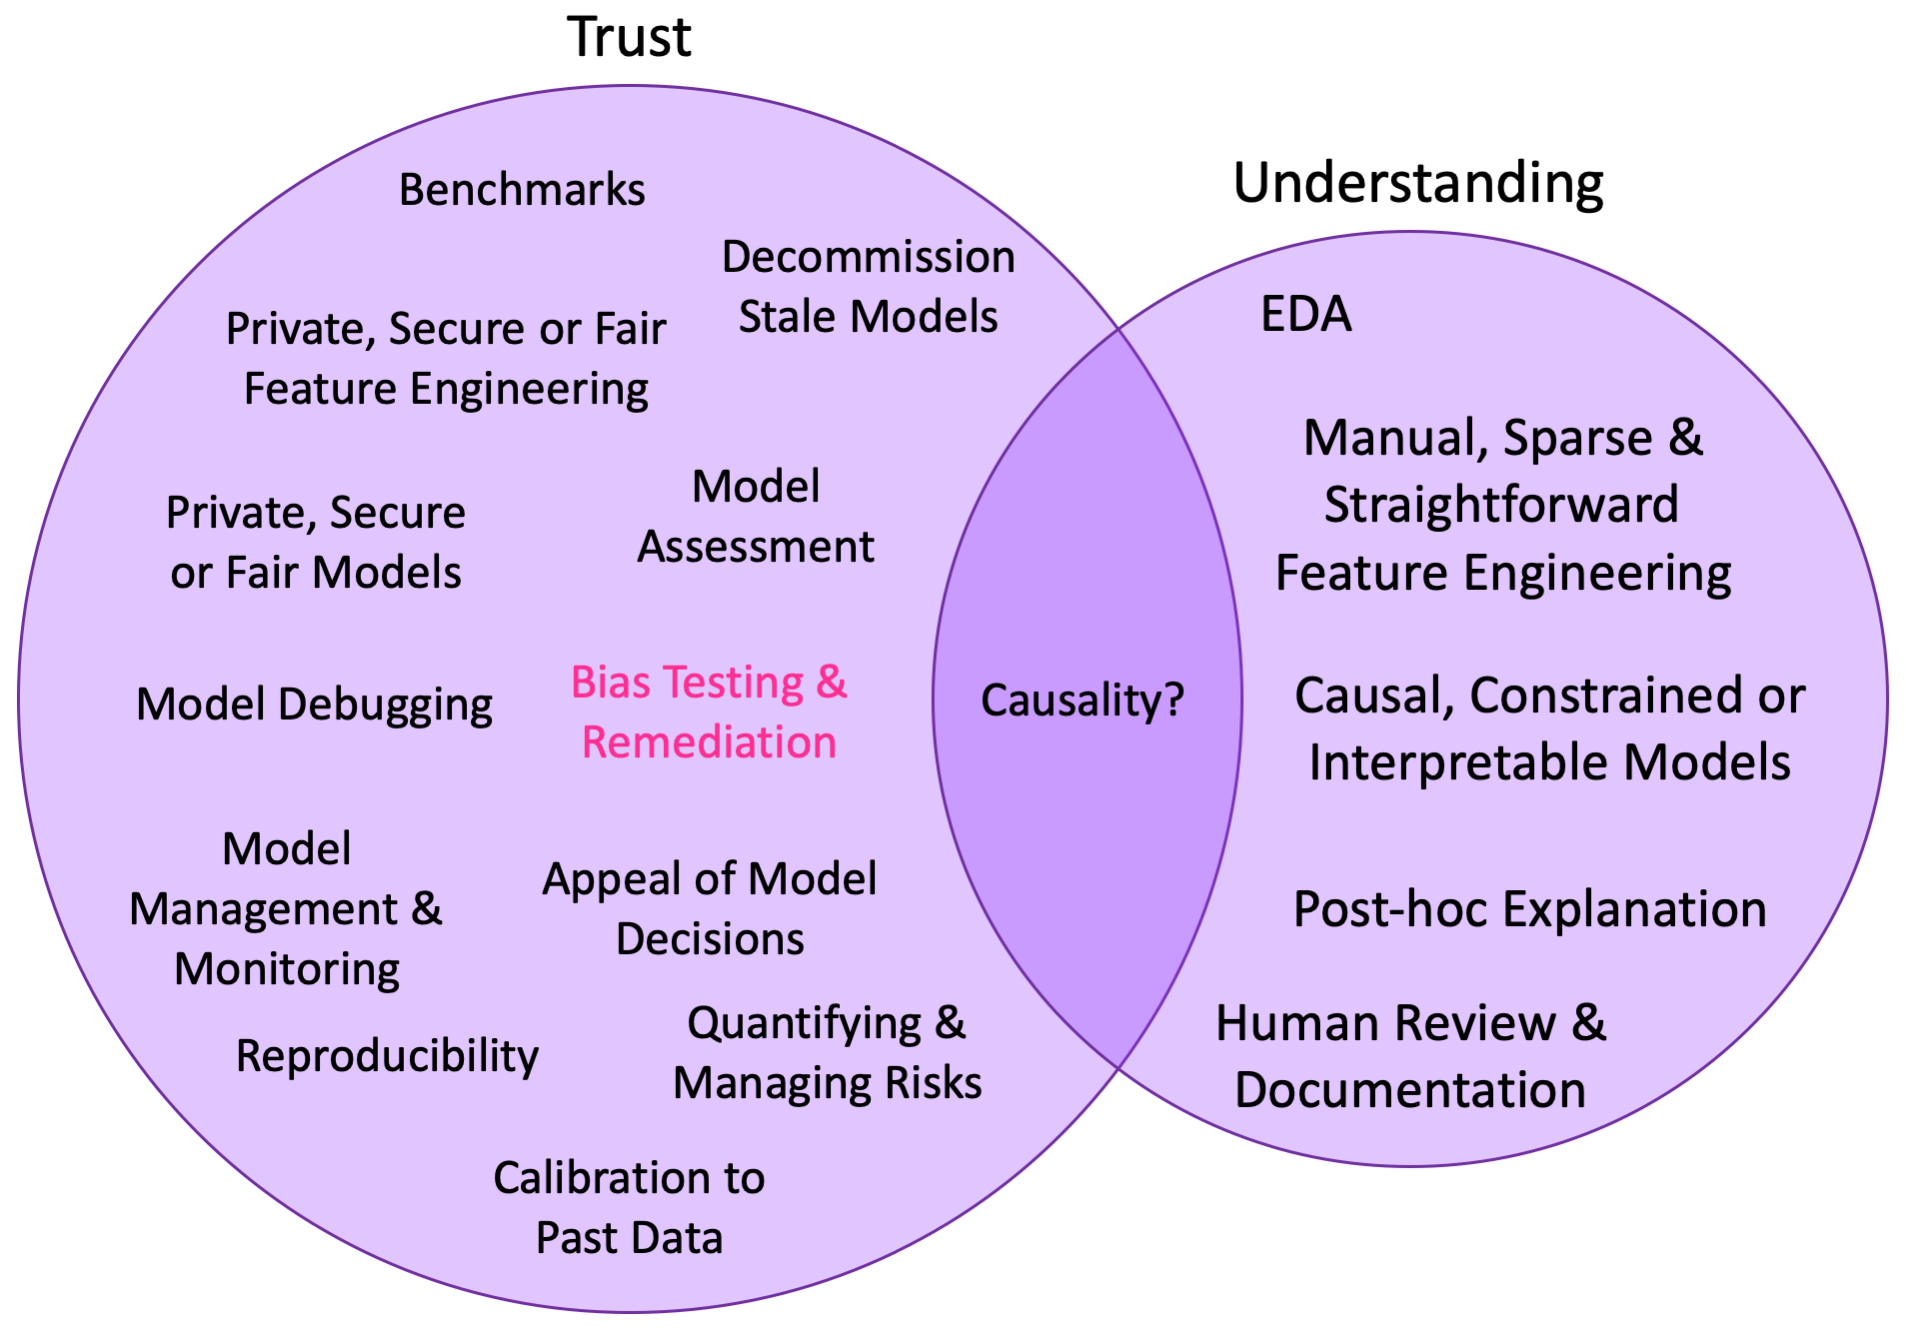
\includegraphics[height=150pt]{../img/trust_understanding.png}
    					\end{center}
  				\end{figure}
  
  				\vspace{-5pt}
  				\scriptsize{Trust and understanding in machine learning are different but complementary goals, and they are technically feasible \textit{today}}.
    
		\end{frame}

%-------------------------------------------------------------------------------
		\subsection{Model Debugging}
%-------------------------------------------------------------------------------	

			\begin{frame}
		
				\frametitle{Model Debugging for Accuracy, Privacy or Security}		
			
				\begin{columns}
	
					\column{0.5\linewidth}
					\centering
					\includegraphics[height=120pt]{../img/md.png}
				
					\column{0.5\linewidth}
					\vspace{-5pt}
					\scriptsize
					{\begin{itemize}
						\item Eliminating errors in model predictions by testing: adversarial examples, explanation of residuals, random attacks and ``what-if'' analysis.
						\item OSS: \href{https://github.com/tensorflow/cleverhans}{cleverhans}, \href{https://github.com/SauceCat/PDPbox}{pdpbox}, \href{https://pair-code.github.io/what-if-tool/index.html}{what-if tool}
						\item References: \citefield{amershi2015modeltracker}{title}; \citefield{papernot2018marauder}{title}; \citefield{security_of_ml}{title}
					\end{itemize}}
					\normalsize
				
				\end{columns}			
			
			\end{frame}
			
			\begin{frame}	
			
				\frametitle{Machine Learning Attacks\footnote{\tiny{See \url{https://github.com/jphall663/secure_ML_ideas} for full size image and more information.}}}		
			
				\begin{figure}[htb]
					\begin{center}
						\includegraphics[height=160pt]{../img/cheatsheet.png}
					\end{center}
				\end{figure}	
			\end{frame}
			

%-------------------------------------------------------------------------------
		\subsection{Post-hoc Disparate Impact Remediation}
%-------------------------------------------------------------------------------					
		
		\begin{frame}		
		
			\frametitle{Post-hoc Disparate Impact Assessment and Remediation}		
			
			\begin{columns}
	
				\column{0.5\linewidth}
				\centering
				\includegraphics[height=120pt]{../img/fair.png}
				
				\column{0.5\linewidth}
				\vspace{-5pt}
				\begin{itemize}
					\item Social bias testing should include group fairness tests and should attempt to consider individual fairness. 
					\item OSS: \href{https://github.com/dssg/aequitas}{aequitas}, IBM \href{https://github.com/IBM/AIF360}{AIF360}, \href{https://github.com/LASER-UMASS/Themis}{themis}
					\item References: \citefield{dwork2012fairness}{title}; \citefield{kamiran2012decision}{title}; \citefield{hardt2016equality}{title}; \citefield{feldman2015certifying}{title} 
				\end{itemize}
				
			\end{columns}
		
		\end{frame}
		
%-------------------------------------------------------------------------------
	\section{Risk}
%-------------------------------------------------------------------------------

		\begin{frame}
		
			\frametitle{Quantify and Plan for Risk}	
			
			\begin{figure}[htb]
				\begin{center}
					\includegraphics[height=135pt]{../img/risk.png}
					\end{center}
				\end{figure}	

			\vspace{-10pt}
			\scriptsize{Your model will be wrong. Stake-holders need to understand and be prepared for the human and financial costs of these wrong decisions.}	
				
		\end{frame}

%-------------------------------------------------------------------------------
	\section{Review}
%-------------------------------------------------------------------------------

		\begin{frame}
		
			\frametitle{Human Review and Documentation}		
			
			\begin{columns}
	
				\column{0.5\linewidth}
				\centering
				\includegraphics[height=120pt]{../img/hr.png}
				
				\column{0.5\linewidth}
				\vspace{-5pt}
				\begin{itemize}
					\item Reference: \citefield{model_cards}{title}
					\item Documentation of considered alternative approaches typically necessary for compliance.
				\end{itemize}
				
			\end{columns}
		
		\end{frame}

%-------------------------------------------------------------------------------
	\section{Deployment}
%-------------------------------------------------------------------------------

		\begin{frame}

			\frametitle{Deployment, Management and Monitoring}		
			
			\begin{columns}
	
				\column{0.5\linewidth}
				\centering
				\includegraphics[height=120pt]{../img/deploy.png}
				
				\column{0.5\linewidth}
				\vspace{-5pt}
				\begin{itemize}
					\item Monitor models for accuracy, disparate impact, privacy violations or security vulnerabilities in real-time; track model and data lineage.
					\item OSS: \href{https://github.com/mlflow/mlflow}{mlflow}, \href{https://github.com/mitdbg/modeldb}{modeldb}, \href{https://github.com/EthicalML/awesome-machine-learning-operations}{awesome-machine-learning-ops metalist}
					\item Reference: \citefield{vartak2016m}{title}
				\end{itemize}
				
			\end{columns}
		
		\end{frame}

%-------------------------------------------------------------------------------
	\section{Appeal}
%-------------------------------------------------------------------------------

		\begin{frame}	
			\frametitle{Human Appeal}		
			
			\begin{figure}[htb]
				\begin{center}
					\includegraphics[height=135pt]{../img/ha.png}
				\end{center}
			\end{figure}	

			%\vspace{-10pt}
			\footnotesize{\textit{Very} important, may require custom implementation for each deployment environment? Related problems exist \href{https://www.nytimes.com/2017/06/13/opinion/how-computers-are-harming-criminal-justice.html}{\textit{today}}}.

		\end{frame}
		
%-------------------------------------------------------------------------------
	\section{Decommission}
%-------------------------------------------------------------------------------

		\begin{frame}	
			\frametitle{Decommission Model}		
			
			\begin{figure}[htb]
				\begin{center}
					\includegraphics[height=135pt]{../img/zde.png}
				\end{center}
			\end{figure}	

			%\vspace{-10pt}
			\footnotesize{When a model becomes absolutely or relatively inaccurate, unfair, or insecure it must be taken out of service, but saved in an executable and reproducible manner.}

		\end{frame}


%-------------------------------------------------------------------------------
	\section{Causality?}
%-------------------------------------------------------------------------------

		\begin{frame}
		
			\frametitle{Causality?}	
			
			\begin{columns}
	
				\column{0.5\linewidth}
				\centering
				\includegraphics[height=120pt]{../img/cause.png}
				
				\column{0.5\linewidth}
				\begin{itemize}
					\item Root cause analysis: can root causes be identified, verified? Formalized into model architecture? 
					\item OSS: \href{https://github.com/microsoft/dowhy}{dowhy}, \href{https://docs.pymc.io/}{pymc3}
					\item References: \citefield{pearl2018book}{title}; \citefield{salvatier2016probabilistic}{title}
				\end{itemize}
				
			\end{columns}
			
		\end{frame}

%-------------------------------------------------------------------------------
	\section{Iterate}
%-------------------------------------------------------------------------------

		\begin{frame}	

			\frametitle{Iterate: Use Gained Knowledge to Improve Accuracy, Fairness, Interpretability, Privacy or Security}		
			
			\begin{figure}[htb]
				\begin{center}
					\includegraphics[height=135pt]{../img/iter.png}
					\label{fig:blueprint}
				\end{center}
			\end{figure}	

			\centering
			Improvements, KPIs should not be restricted to accuracy alone.
		
		\end{frame}

%-------------------------------------------------------------------------------
%	\section{Questions}
%------------------------------------------------------------------------------

%		\begin{frame}

%			\frametitle{Open Conceptual Questions}		

%			\begin{itemize}
%				\item How much automation is appropriate, 100\%?
%				\item How to automate learning by iteration, reinforcement learning?
%				\item How to implement human appeals, is it productizable?
%			\end{itemize}
			
%		\end{frame}

%-------------------------------------------------------------------------------
%	References
%-------------------------------------------------------------------------------

	\begin{frame}[t, allowframebreaks]
	
		\frametitle{References}	
		
			\textbf{These slides:}\\
			\small{\url{https://github.com/jphall663/hc_ml}}
			
			\vspace{10pt}
			
			\textbf{"Awesome" Machine Learning Interpretability Resource List:}\\
			\small{\url{https://github.com/jphall663/awesome-machine-learning-interpretability}}
		
		\framebreak		
		
		\printbibliography
		
	\end{frame}

\end{document}